\chapter{Evaluation}
\label{Evaluation}

\begin{flushright}{\slshape    
Statistics are a little like anarchists: \\
if you force them to stay in line, you're begging for trouble.} \\ \medskip
    --- Sarah Slobin, Graphics Editor, The Wall Street Journal
\end{flushright}

\marginpar{Parts of this chapter have previously appeared in \cite{Niezen2012}.}

In this chapter, two evaluations are described. First we will look at an evaluation of the system performance of the software architecture. This evaluation was performed during the smart home pilot of the second design iteration described in Chapter \ref{DesignIteration2}. Secondly, we will look at a method the author developed to evaluate ontologies based on the \ac{CD} framework, as well as an evaluation of the ontology described in this thesis using the method.\marginpar{The \ac{CD} framework was first mentioned in Section \ref{autohan}.}

\section{Evaluating the system performance}
\label{performance}
%SeNAmI start
\subsection{Introduction}

To evaluate the software architecture described in Chapter \ref{SoftwareArchitecture}, we compared it against a previous evaluation of the two M3-based smart space implementations, Smart-M3 and \ac{RIBS}, described in Section \ref{m3}. These implementations were evaluated by Etel\"aper\"a et al \cite{Etelapera2011}. They performed both a qualitative evaluation and quantitative measurements. The performance measurements were made on a Intel Atom 1.6GHz laptop connected via a 100Mbps Ethernet router to a Intel Pentium M 1.7GHz laptop. The qualitative evaluation focused on documentation, installation process and portability as well as run-time usability. According to \cite{Etelapera2011} \ac{RIBS} is up to 237 times faster than Smart-M3 in certain instances, but it is reported that its memory model limits the number of use cases it can be applied to. \ac{RIBS} uses static memory allocation with no disk storage and a bitcube triple store, which means that the maximum number of triples has to be known a priori.

Query time measurements for Smart-M3 indicated a query time of 4.4ms for one triple and 8.6ms for 10 triples. For \ac{RIBS} a query time of 0.65ms was measured for one triple. \ac{RIBS} did not support querying 10 triples at the time the evaluation was performed. Subscription time measurements indicated a subscription indication time of 140ms for Smart-M3, while \ac{RIBS} measured 0.75ms.

Bhardwaj et al. \cite{Bhardwaj2011} compared Smart-M3 against their \ac{OSAS} framework. They did a performance analysis based on end-to-end delay measurements between the smart objects in smart spaces. The analysis shows that the end-to-end delays are mostly dominated by KP-to-SIB updates, rather than the processing delays on \acp{KP} or on the \ac{SIB}.

% A number of ontologies have been developed for ubiquitous computing environments. Chen et al. \cite{chen2004} defined SOUPA, a context ontology based on OWL (Web Ontology Language), to support ubiquitous agents in their Context Broker Architecture (CoBrA). The ontology supports describing devices on a very basic level (e.g. typical object properties are \texttt{bluetoothMAC} or \texttt{modelNumber}), but it has no explicit support for modeling more general device capabilities.

% Ngo et al. \cite{Ngo2004} developed the CAMUS ontology in OWL to support context awareness in ubiquitous environments. Their device ontology is based on the FIPA device ontology specification\footnote{http://www.fipa.org/specs/fipa00091/SI00091E.html}. Unfortunately it does not define a notion of completeness, and the ontology is thus not considered generic enough for general use in ubicomp environments.

Luukkala et al. \cite{Luukkala2010} used Smart-M3 with \ac{ASP} techniques to handle resource allocation and conflict resolution. They used the \ac{SPICE} Mobile Ontology\footnote{http://ontology.ist-spice.org/} to describe device capabilities and \ac{ASP} as a rule-based approach to reasoning. The \ac{SPICE} ontology allows for the definition of device capabilities in a sub-ontology called \ac{DCS} \cite{Villalonga2009}.\marginpar{The \ac{SPICE} \ac{DCS} ontology was first mentioned in Section \ref{spice}.}

%While the ontology provides for a detailed description of the different modality capabilities, e.g. being able to describe force feedback as a \texttt{TactileOutputModalityCapability}, there are no subclass assertions made for other device capabilities.

%This could be extended with work from Riboni et al; Liming Chen (and maybe Sabou's paper)

\subsection{Experimental setup}
\label{implementation}

% The software framework that was used to implement the system is based on the SOFIA IOP. SOFIA\footnote{http://www.sofia-project.eu/} (Smart Objects For Intelligent Applications) is an European research project within the ARTEMIS framework that attempts to make information in the physical world available for smart services - connecting the physical world with the information world. The SOFIA IOP uses a blackboard architectural model that implements the ideas of space-based computing \cite{Honkola2010}. It consists of two main components: a SIB (Semantic Information Broker) that acts as a common, semantic-oriented store of information and device capabilities, and KPs (Knowledge Processors), virtual and physical smart objects that interact with one another through the SIB. Various SIB implementations exist that conform to the M3 specification, of which Smart-M3 was the first open source reference implementation released in 2009\footnote{http://sourceforge.net/projects/smart-m3/}. RIBS (RDF Information Base System) is a C-based implementation of M3 targeted for devices with low processing power, but requires a high amount of memory \cite{Etelapera2011}.  The SIB implementation used in the pilot is called ADK-SIB (Application Development Kit SIB) and was developed within the SOFIA project. 

%The system architecture of the implementation of the smart home pilot is shown in Figure \ref{pilot}.
% The smart home pilot follows the following scenario:
% 
% \textit{Mark and Dries enter their home. The intelligent lighting system (Presence KP) detects their presence, and switches the lights on, and notifies the smart space about user presence. The decorative wall-wash lights (Lamp KP) are in turn notified of user presence by the smart space, and turn themselves on. Mark and Dries start listening to music (Music Player KP). They would like to try to render the music on a lighting device to also create some visual effects accompanying the music. They query the smart space and find out that the lighting device can render these light effects (using the Sound/Light Transformer KP). They make a connection between the music player and the lighting device using the Connector (Connector KP). The light is rendered on the lighting device. To put the focus on the lighting device, the decorative wall-wash lights in the room automatically dim themselves down. At the same time, the light pattern also starts being rendered on the remote lighting device, where Mark's sister Sofia can observe the same light effects in her own house.}
% 
% \textit{At another location: after a while, Sofia is curious and wants to listen to the music that Mark and Dries are listening to. She connects her lighting device to her stereo, and the same song plays on her surround sound system (remote Music Player KP).}
% --Note: Since we don't mention spotlight navigation elsewhere, Sachin suggested we remove it from the scenario

%She uses the spotlight navigation device to make a connection from the bonding device to the stereo. When she starts using the spotlight navigator, the lights in the room dim down to enhance the visibility of the spotlight. Once the connection is made, the lights go back up.


% \begin{figure}
% \centering
% \includegraphics[width=250px]{pilot}
% \caption{System architecture of the Smart Home Pilot}
% \label{pilot}
% \end{figure}
\marginpar{The smart home pilot scenario was first described in Section \ref{D2Requirements}.}
In the smart home pilot, media content is shared among several devices in a smart home setting. Music is shared between a mobile device, a stereo speaker set and a lighting device that renders the mood of the music with coloured lighting. The music experience, consisting of both light and music information, is also shared remotely between friends living in separate homes through the lighting device. Other lighting sources, like the smart functional lighting and the smart wall wash lights are sensitive to user presence and the use of other lighting sources in the environment.

\marginpar{An overview of the smart home pilot is shown in Figure \ref{pilotSetup} on page \pageref{pilotSetup}, while a diagram showing the technical details is shown in Figure \ref{SmartHomePilotDiagram} on page \pageref{SmartHomePilotDiagram}.} The performance measurements were made in an environment that approximates a real-world home environment for these kinds of devices. Two wireless routers were placed in two different locations, bridged with an ethernet network cable. One router was configured to act as a DHCP server, while the other acted as a network bridge. The Connector \ac{KP}, Music Player \ac{KP} and \ac{SIB} were connected to the router in location A, while the \ac{SLT} KP was connected to the router in location B. All components were connected to the network via the 802.11g wireless protocol. The system specifications of each component used in the performance evaluation are shown in Table \ref{specs}.


\begin{table}\footnotesize
    \myfloatalign
  \begin{tabularx}{\textwidth}{lllll} 
	\toprule
    \tableheadline{Component} & \tableheadline{CPU} & \tableheadline{OS} & \tableheadline{Memory} & \tableheadline{Language} \\ 
    \midrule

	SIB & Core 2 Duo 2.8GHz & Ubuntu 10.04 & 4GB & Java \\
	SLT KP & Core 2 Duo 2.2GHz & Ubuntu 11.04 & 2GB & Java\\
	Connector KP & Core 2 Duo 2.6GHz & OS X 10.6.8 & 4GB & Python\\
	Music Player KP & ARM Cortex-A8 & Maemo 5 & 256MB & Python\\
	Presence KP  & Pentium M & Ubuntu 10.04 & 512MB & Python\\
	Lamp KP  & Pentium M & Ubuntu 10.04 & 512MB & Python\\
	
    \bottomrule
  \end{tabularx}
  \caption{System specifications of components used in evaluation}\label{specs}
\end{table}
% OMAP 3430

Figure \ref{soundLight} and Figure \ref{connectorseq} show the sequence diagrams of the measurements made for the \ac{SLT} \ac{KP} and the Connector \ac{KP} respectively. During the pilot, 86 measurements were made by the \ac{SLT} \ac{KP} -- each time an event was received. 961 measurements were made by the Connector \ac{KP} -- each time a user scans a tag. Note that the query name in \ref{connectorseq} could differ between subsequent queries, as the user could be scanning a different tag every tames.

\begin{figure}
\centering
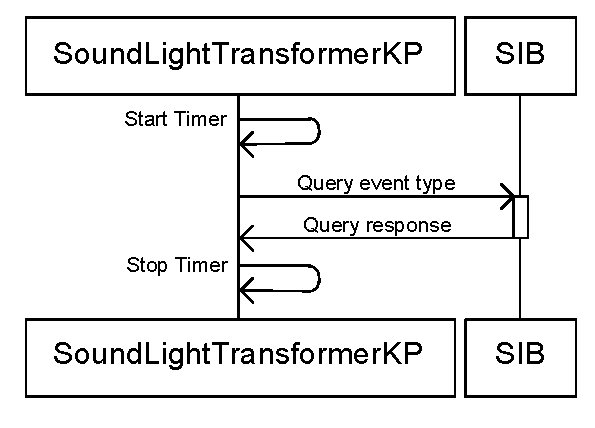
\includegraphics[width=200px]{soundLight}
\caption{Sequence diagram of Sound/Light Transformer KP query measurement}
\label{soundLight}
\end{figure}

\begin{figure}
\centering
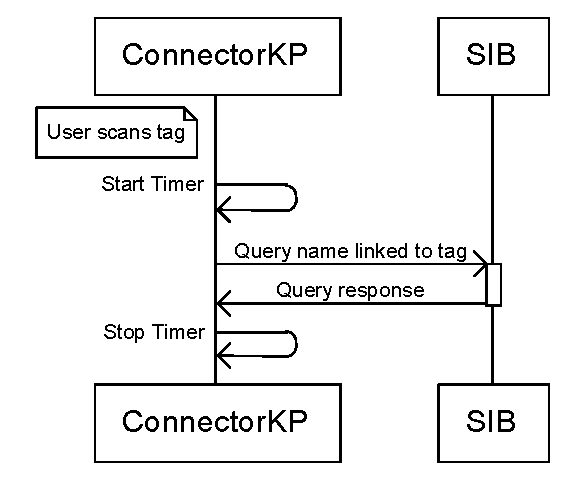
\includegraphics[width=200px]{connectorseq}
\caption{Sequence diagram of Connector KP query measurement}
\label{connectorseq}
\end{figure}

For the music player \ac{KP}, we measured the time between inserting a new event, and receiving an update from the \ac{SIB} indicating that the specific event had occurred. First a subscription is made to the \texttt{PlayEvent} type, as shown in Figure \ref{N900}. A new \texttt{PlayEvent} is generated by the \ac{KP}, and when the \ac{KP} is notified of this event by the \ac{SIB}, the \ac{KP} queries the \ac{SIB} to determine if the notification is indeed for the event that it generated itself.

The Lamp-KP was connected to the decorative wall-wash lights (four LED lamps), creating coloured illumination on the wall of the room. The lamps are shown in Figure \ref{lamp-KP}, including a description of its components. The Presence-KP  determines the presence of a user in an activity area of a room and sends the presence information to the SIB. The Lamp-KP is subscribed to this presence information, and gets updated whenever the presence is updated by the Presence-KP to the \ac{SIB}. There are two states to be updated by the Presence-KP on the \ac{SIB}: \texttt{Away} and \texttt{Present}. Based on these states, the Lamp-KP turns the lamps on or off. For example, when the \texttt{Present} state is specified by the Presence-KP, the Lamp-KP sends  the \texttt{ON} command to all lamps, and the \texttt{OFF} command when the \texttt{Away} state is specified.  The Lamp-KP is also subscribed to the states of the \ac{SLT} KP. The sequence diagram for the Presence-KP, \ac{SLT} KP, Lamp-KP and \ac{SIB} is shown in Figure \ref{sequence-lamp}.

%When music starts rending then the Lamp-KP sends DIM command to the lamps. 

\begin{figure}[bth]
\centering
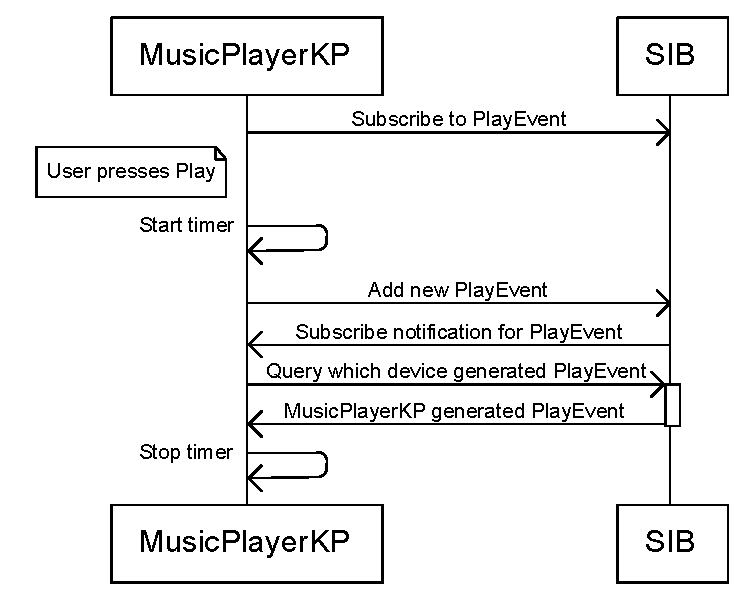
\includegraphics[width=250px]{n900}
\caption{Sequence diagram of Music Player KP subscription measurement}
\label{N900}
\end{figure}

\begin{figure}[bth]
\centering
%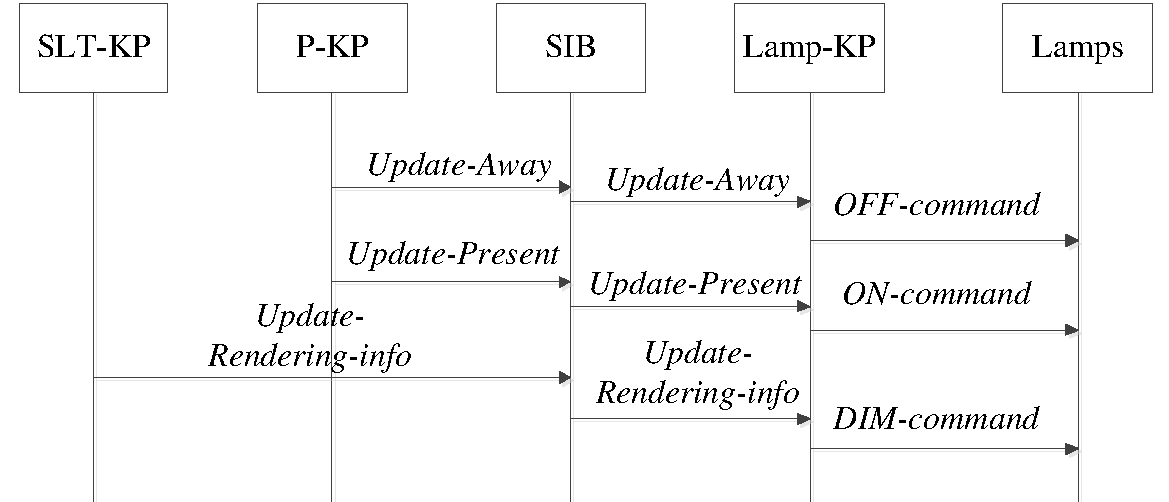
\includegraphics[width=\textwidth]{sequence-lamp}
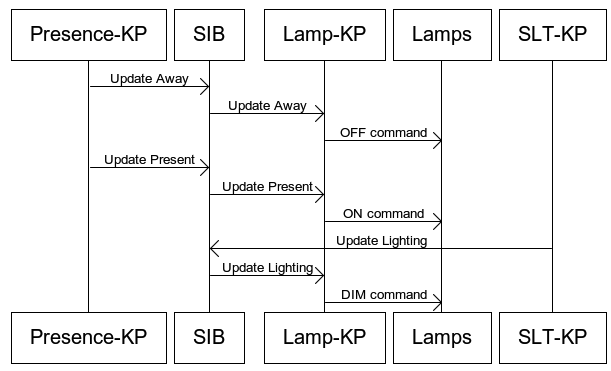
\includegraphics[width=300px]{lampseq}
\caption{Sequence diagram of Presence-KP and Lamp-KP}
\label{sequence-lamp}
\end{figure}


% \begin{figure}[bth]
% \begin{msc}
% msc {
% 	//hscale = "1.5";
% 	
%     slt [label="SLT-KP"], p[label="Presence-KP"], sib [label="SIB"], lamp [label="Lamp-KP"], lamps [label="Lamps"];
% 
% 	p->sib [label="Update Away"];
% 	sib->lamp [label="Update Away"];
% 	lamp->lamps [label="OFF command"];
% 	p->sib [label="Update Present"];
% 	sib->lamp [label="Update Present"];
% 	lamp->lamps [label="ON command"];
% 	slt->sib [label="Update Lighting"];
% 	sib->lamp [label="Update Lighting"];
% 	lamp->lamps [label="DIM command"];
% }
% \end{msc}
%         \caption{Sequence diagram of Presence-KP and Lamp-KP}
%         \label{sequence-lamp}
% \end{figure}

\begin{figure}[bth]
\centering
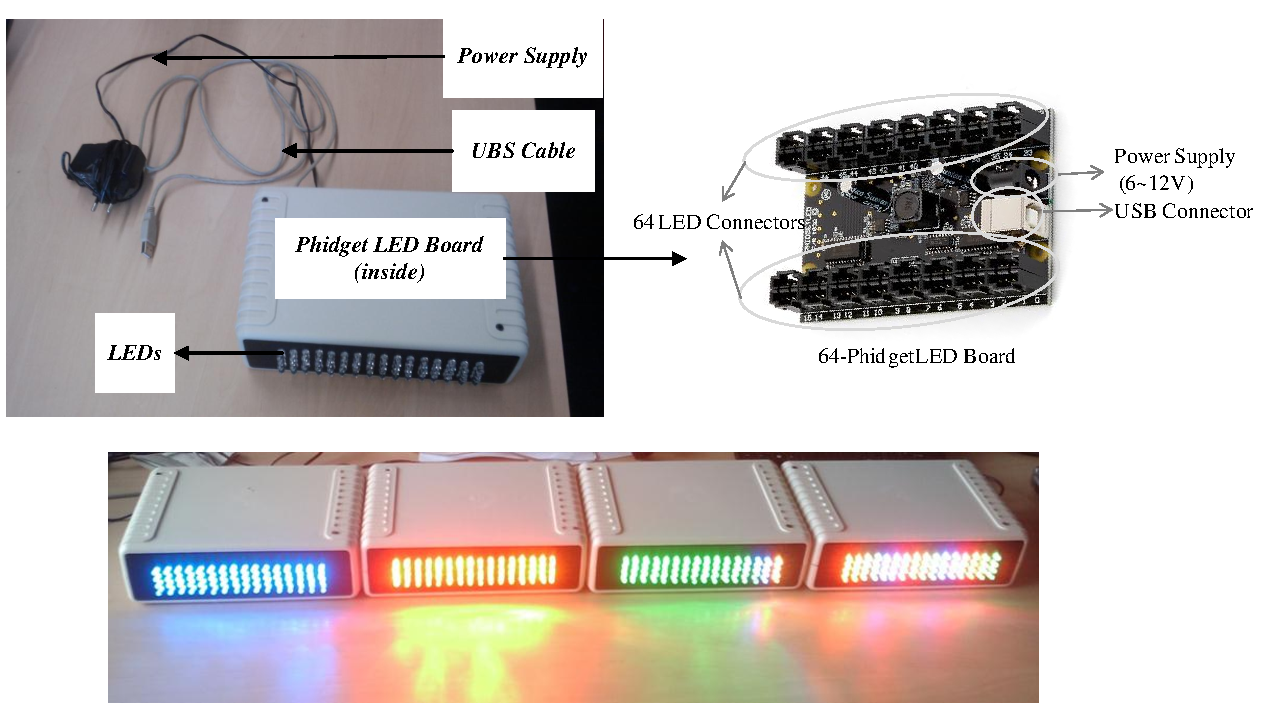
\includegraphics[width=300px]{lamp-KP}
\caption{Lamp-KP}
\label{lamp-KP}
\end{figure}

% \subsubsection{Performing reasoning with the SIB}
% 
% Reasoning on information contained within the SIB was performed using OWL 2 RL and SPIN (See Section \ref{SPIN}).  OWL inferences for OWL 2 RL were executed by using SPIN rules. For more information on OWL 2 RL and SPIN, see Section \ref{owl2rl}.
% 
% When the SPIN engine is started (we use the open source TopBraid SPIN API), it iterates until there are no new triples constructed - we call this one \emph{reasoning cycle}. Existing inferences from a previous reasoning cycle are cleared before each new reasoning cycle. Triples that were previously inferred (based on a CONSTRUCT SPIN rule), are removed when the asserted triple (which caused the inferred triple) does not exist anymore. Triples are inferred (using SPIN rules) when new triples are inserted by devices connected to a triple store. For example, consider a device inserting a \texttt{sc:connectedTo} relationship when it is connected to another device. When the asserted triples are later removed by these devices (e.g. a device removing its \texttt{sc:connectedTo} relationship when the other device disconnects), the triples that were inferred based on these triples should be removed as well.

\subsubsection{Reasoning setup}

For the pilot, constraint violation checking was disabled, as this introduced quite a large delay ($>1000ms$), and was not necessary for the purposes of the pilot. Constraint checking ensures that instances in the triple store meet the constraints attached to classes and properties in an ontology. Constraint violation checks are computationally expensive and cannot be performed for each add, remove and update operation. One possible solution is to perform constraint violation checks at regular intervals and then remove the offending triples.

% \subsubsection{OWL 2 RL and SPIN}
% \label{owl2rl}
% 
% An example of where an OWL 2 property chain is used to perform semantic matching of media types is shown as:\\
% 
% 
% \noindent
% transmitsMediaType~\ensuremath{\circ}~isAcceptedMediaTypeOf\\~\ensuremath{\sqsubseteq}~convertsMediaType\footnote{The concatenation of two relations $R$ and $S$ is expressible by $R \circ S $, while $ R \sqsubseteq S$ indicates that $R$ is a subset of $S$ }\\
% 
% 
% This is modelled in the ontology as:
% \usemintedstyle{manni}
% \begin{minted}[fontsize=\footnotesize]{turtle}
% sc:convertsMediaType
% 	a owl:ObjectProperty; 
% 	a owl:IrreflexiveProperty ;
%     owl:propertyChainAxiom
%     	(sc:transmitsMediaType 
% 		 sc:isAcceptedMediaTypeOf) .
% \end{minted}

% (moved to OntologyEngineering)
% We realized early on that some kind of rule-based functionality will be required in addition to the functionality provided by an ontology language like OWL 2. Originally we considered using SWRL (Semantic Web Rule Language) \cite{Niezen2011}, but it was deemed not expressive enough. Due to it being a DL (Description Logic)-safe language, it is not possible to create new individuals based on inferences. With SPARQL, this is possible using a CONSTRUCT query, defined as a SPIN rule as shown in Listing \ref{constructspin}.
% 
% 
% \begin{figure*} % \begin{listing} does not seem to support twocolumn
% % to use sparl lexer, install https://github.com/gniezen/n3pygments	
% \begin{minted}[linenos,
%                numbersep=5pt,
%                %gobble=2,
%                frame=lines,
%                fontsize=\footnotesize,
%                framesep=2mm]{sparql} 
% CONSTRUCT {
%     ?mp a sc:MediaPath .
%     ?x3 sc:hasMediaPath ?mp .
%     ?mp bonding:mediaSourceSO ?x2 .
%     ?mp bonding:mediaOriginator ?this .
% }
% WHERE {
%     ?this sc:convertsMediaType ?x2 .
%     ?x2 sc:convertsMediaType ?x3 .
%     ?this sc:connectedTo ?x3 .
%     BIND (IRI(fn:concat("example.com/ontology#mediaPath_", afn:localname(?this),
%      "_to_",afn:localname(?x3))) AS ?mp) .
% }
% \end{minted} 
% \captionof{listing}{Creating a new individual using SPARQL CONSTRUCT and SPIN} 
% % see http://tex.stackexchange.com/a/12430/8419
% \label{constructspin}
% \end{figure*}
% 
% In the example, a new \texttt{mediaPath} individual is created if two smart objects are connected to each other and there is a \texttt{mediaSourceSO} (semantic transformer) that converts the media types between them. This could be a media player transmitting music as source, an ambient lighting object that accepts RGB colour values as sink, and a semantic transformer that converts audio streams into RGB lighting information. For more information about media paths and semantic transformers, see \cite{Niezen2011}.
% 
% The \texttt{?this} variable indicates to SPIN how the definition should be applied to the members of a class, as the rule itself is defined as part of the class definition - thus defining the scope of the query. \texttt{fn:concat} and \texttt{afn:localname} are SPIN functions used to concatenate the name of the individual and retrieve the local names of the variables used respectively.

% Although SWRL is supported by the Pellet and HeRMiT reasoners, it is not yet standardized and has stayed a W3C Member Submission\footnote{http://www.w3.org/Submission/SWRL/} since 2004. SPARQL is a W3C Recommendation, actively developed and well supported by the Semantic Web community.

We made use of OWL 2 RL/RDF Rules in the smart home pilot, which is a \emph{semantic} subset of OWL 2 \emph{Full}. This should not be confused with the first part of the OWL 2 RL Profile\footnote{http://www.w3.org/TR/owl-profiles/}, which is a \emph{syntactic} subset of OWL 2 \emph{DL}, and restricted in the type of inferences that can be performed. In practice, most OWL 2 reasoners implement OWL 2 RL/RDF Rules (from here on known as OWL 2 RL). OWL 2 RL addresses a significant subset of OWL 2, including property chains and transitive properties. It is fully specified as a set of rules - in our case, as a set of \ac{SPIN} rules. This means that it is even possible to select only the parts of OWL 2 that are required for a specific ontology, to allow for scalable reasoning.
% Could add info about tractability

During the smart home pilot, all \ac{SSAP} messages received by the \ac{SIB} were logged for further analysis.\marginpar{\ac{SSAP} is described in Section \ref{ssap}.}

\subsection{Experimental Results}
\label{results}

After every reasoning cycle both the asserted and inferred models were written to disk, generating a total of 8306 models during the pilot. Reasoning was performed once, after all ontologies were loaded, and then for every add, remove and update operation. This resulted in a total of 5158 measurements of model size and reasoning time during the pilot. No reasoning was performed during queries.

During the pilot, 70655 total queries were performed by devices connected to the \ac{SIB}. The time to perform each query was recorded on the \ac{SIB}, and is shown in Figure \ref{querytime}. The histogram with bin size 25 is plotted on a logarithmic scale. Around 70000 queries take 2ms or less to complete, accounting for more than 99\% of the queries. Of all the queries, only 3 queries took 30ms or longer to complete, with all queries completing in less than 60ms. Keep in mind that these measurements were performed on the \ac{SIB}, hence the measurements do not take network latency into account.

\begin{figure}
\centerline{
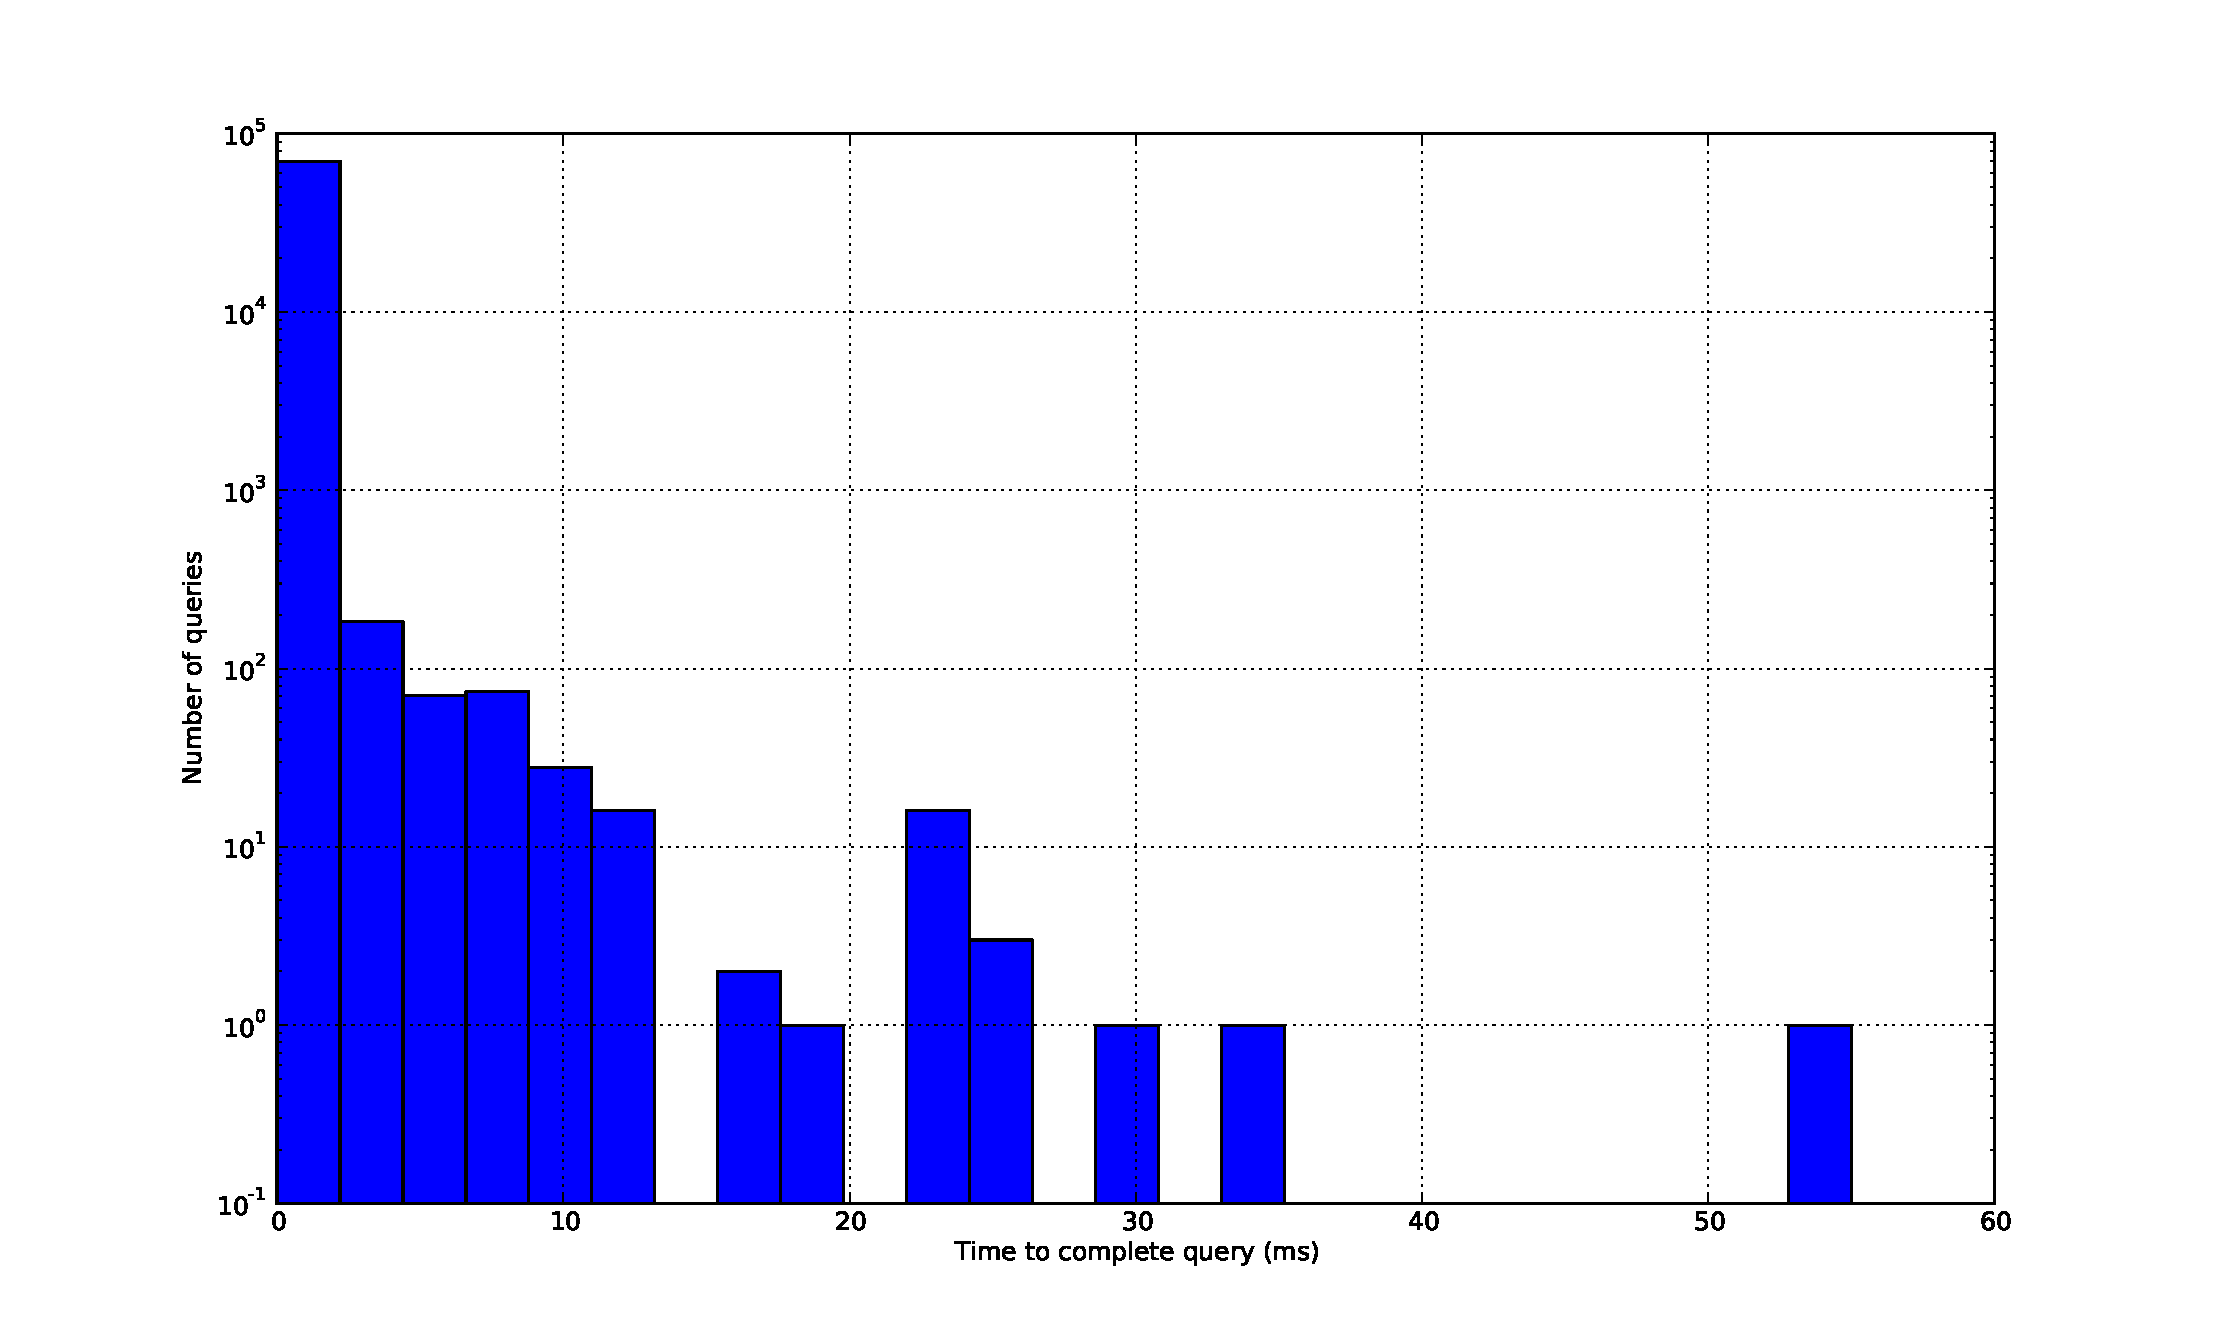
\includegraphics[width=500px]{querytime}}
\caption{Query time measurements on SIB}
\label{querytime}
\end{figure}

Figure \ref{kdeplot} shows the histograms, Gaussian \acp{KDE} and \acp{CDF} of the Connector \ac{KP} and \ac{SLT} \ac{KP} \emph{query time measurements}. A bin size of 20 and a bandwidth of 0.5 was used to plot the figures. It shows that the typical query time for the Connector \ac{KP} is very short, with a few outliers that took a very long time to complete (35.2s). For the \ac{SLT} \ac{KP}, the case is similar, but there are no extreme outliers, with the longest query taking only 587ms to complete. Note that the \ac{KDE} provides similar information to the histogram, but handles outliers more gracefully by not using binning, and also results in a smoother graph.

The \ac{CDF} of the Connector \ac{KP} indicates that queries taking more than two seconds to complete are very rare. The queries that do take longer than two seconds, take an unusually long time to complete. We believe that it could be related to problems in the wireless network, or related to the Python implementation of the \ac{KPI}, as the problem did not present itself when using other \ac{KPI} implementations.

For the \ac{SLT} \ac{KP}, most queries completed within 100ms, with very few queries taking longer than 500ms to complete.

\begin{figure}
\centerline{
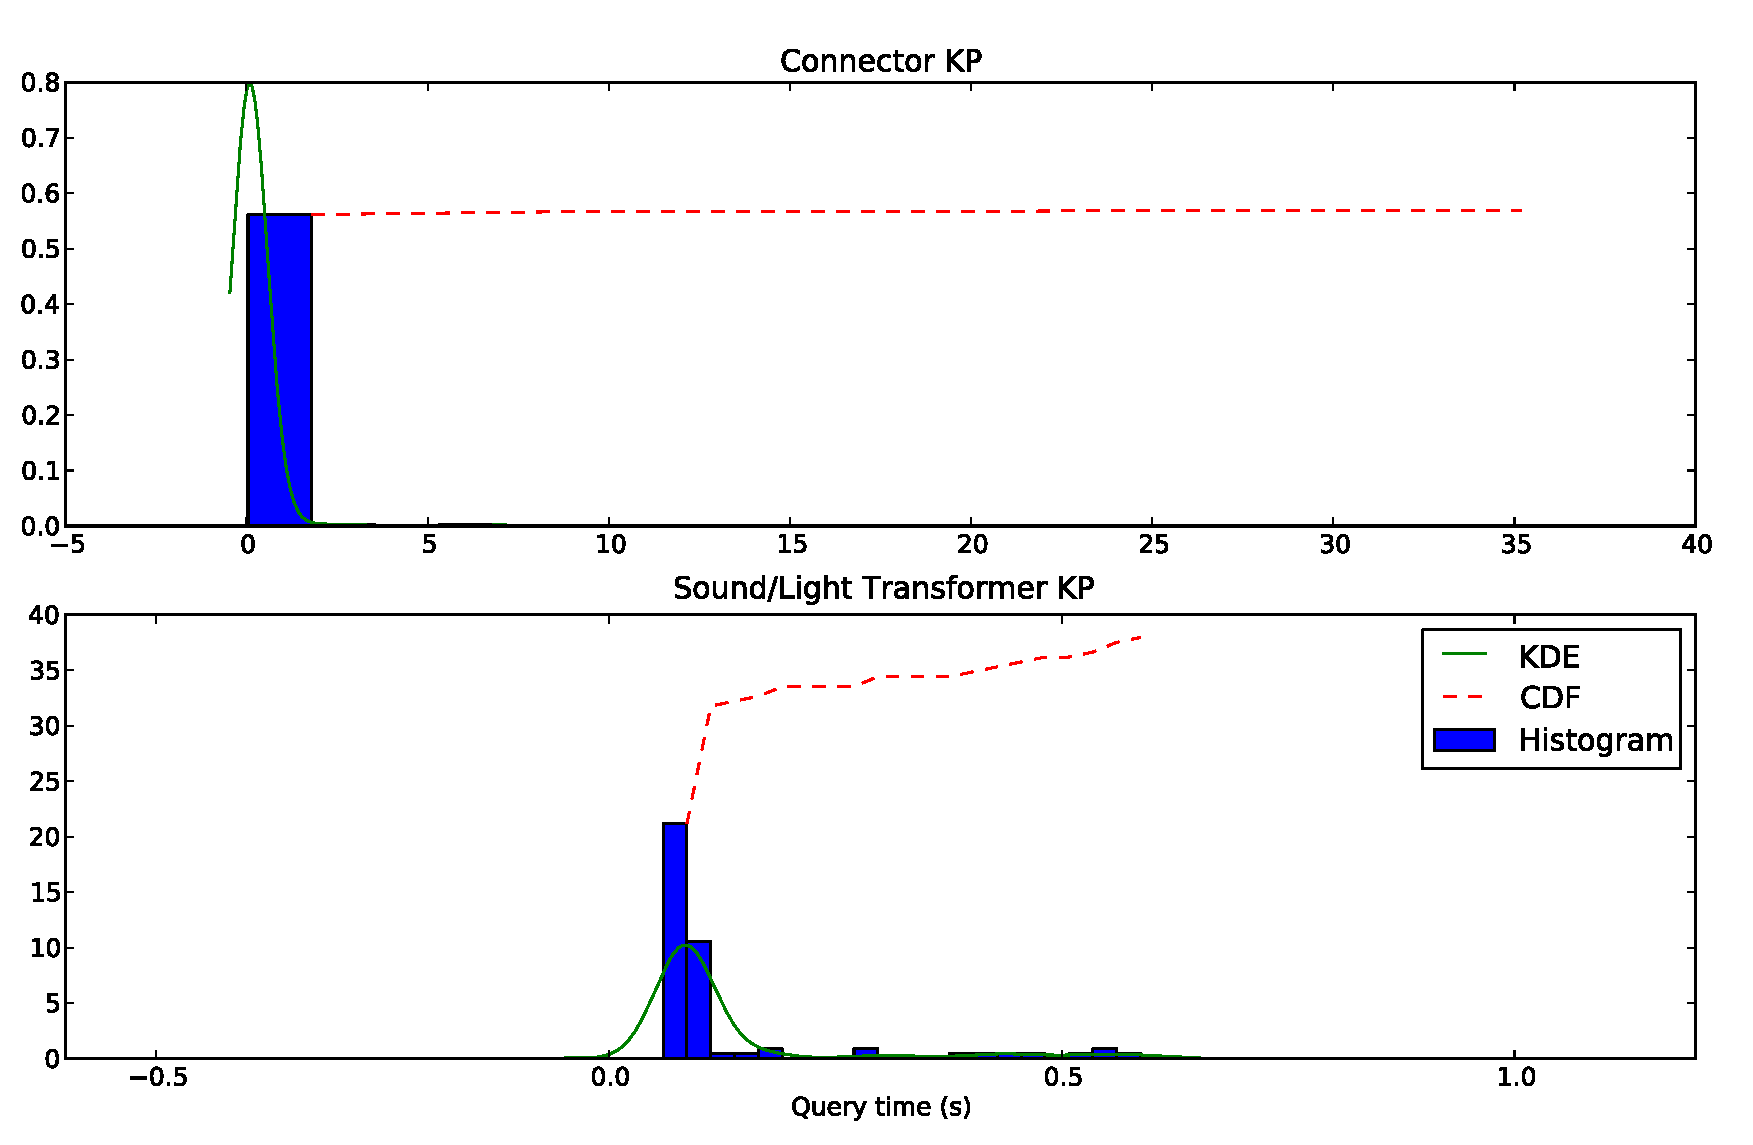
\includegraphics[width=400px]{kdeplot2}}
\caption{Histograms, kernel density estimates and cumulative distribution functions of Connector KP and Sound/Light Transformer KP measurements}
\label{kdeplot}
\end{figure}

For the music player \ac{KP}, most subscription notifications completed in an average of 0.86s, as shown in Figure \ref{n900plot}. Keep in mind that after the new PlayEvent is added, inferencing is performed on the triple store before the subscribe notification is generated. Summary statistics of Music Player \ac{KP}, Connector \ac{KP} and Sound/Light Transformer \ac{KP} measurements are shown in Table \ref{summaryKP}.

\begin{figure}
\centerline{
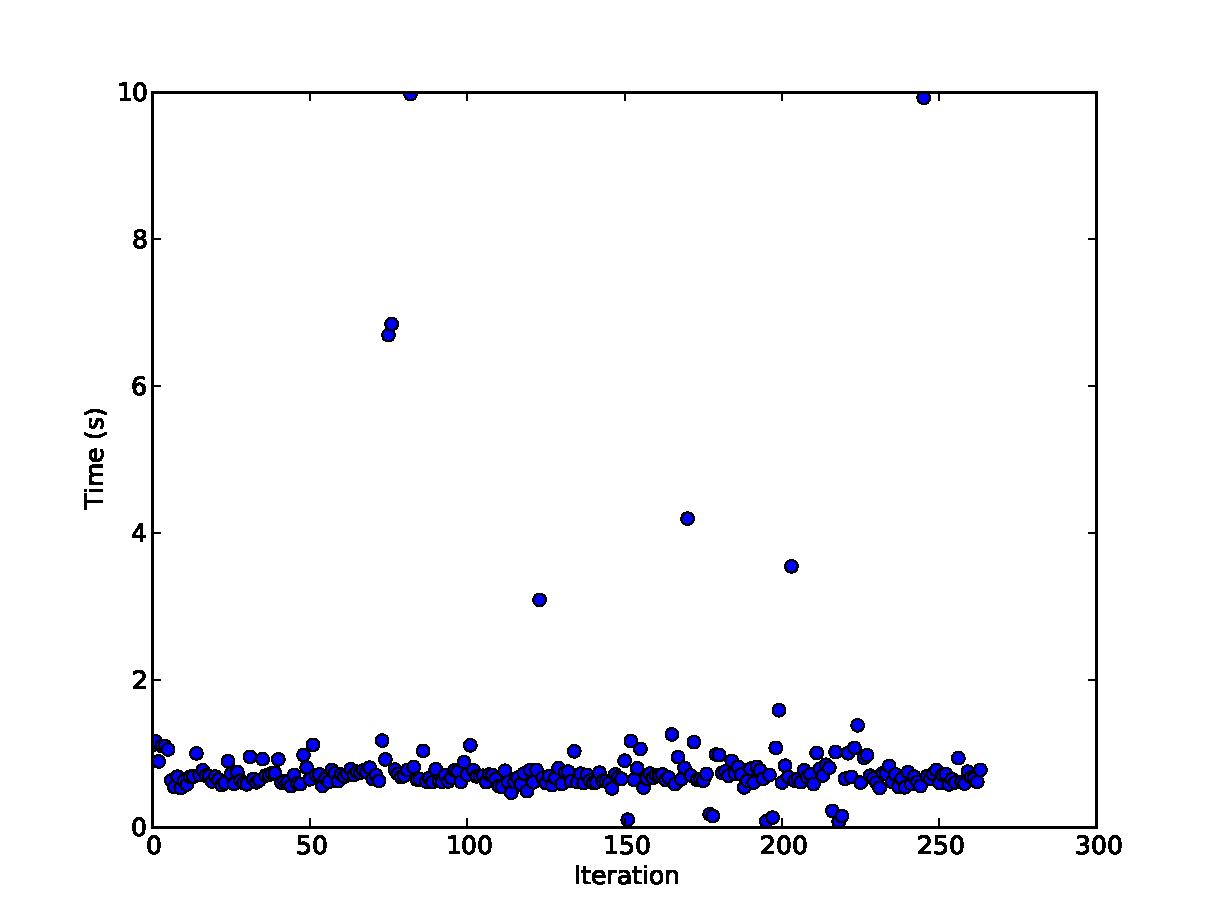
\includegraphics[width=400px]{n900plot}}
\caption{Subscription measurements of Music Player KP}
\label{n900plot}
\end{figure}


\begin{table}
    \myfloatalign
  \begin{tabularx}{\textwidth}{llllll} 
	\toprule
    \tableheadline{Component} & \tableheadline{Nr. of obs.} & \tableheadline{Min.} & \tableheadline{Max.} & \tableheadline{Mean} & \tableheadline{Std. dev.} \\ 
    \midrule

	Music Player KP & 264 & 0.074 & 9.975 & 0.861 & 1.017\\
	Connector KP & 961 & 0.044 & 35.184 & 0.275 & 1.942\\
	Sound/Light KP  & 86 & 0.06 & 0.587 & 0.131 & 0.122 \\
	Lamp-KP & 98 & 0.012 & 0.049 & 0.03 &0.006 \\
	Presence-KP & 172 & 0.145 & 0.244 & 0.176 & 0.018 \\
	
    \bottomrule
  \end{tabularx}
  \caption{Summary statistics of Music Player KP, Connector KP and Sound/Light Transformer KP measurements}\label{summaryKP}
\end{table}


In Figure \ref{stats}, the following is shown:
\begin{itemize}
\item Model size: Number of triples asserted by ontology or connected KPs
\item Inferred model size: Number of triples inferred by reasoning engine
\item Inferencing duration: Time (in ms) to complete one reasoning cycle
\end{itemize}

The sharp peaks indicate the times that the SIB was restarted. The first reasoning cycle after a restart takes about 3 seconds,  with subsequent cycles taking on average 275ms (as seen in Table \ref{summarySIB}).

There is a slow but steady increase in the number of triples as new events get added to the triple store. After each restart these events are cleared and the base assertions loaded from the ontology. These assertions include the OWL 2 RL specification, stored as SPIN rules, which account for the large number of triples.

\begin{figure}
\centerline{
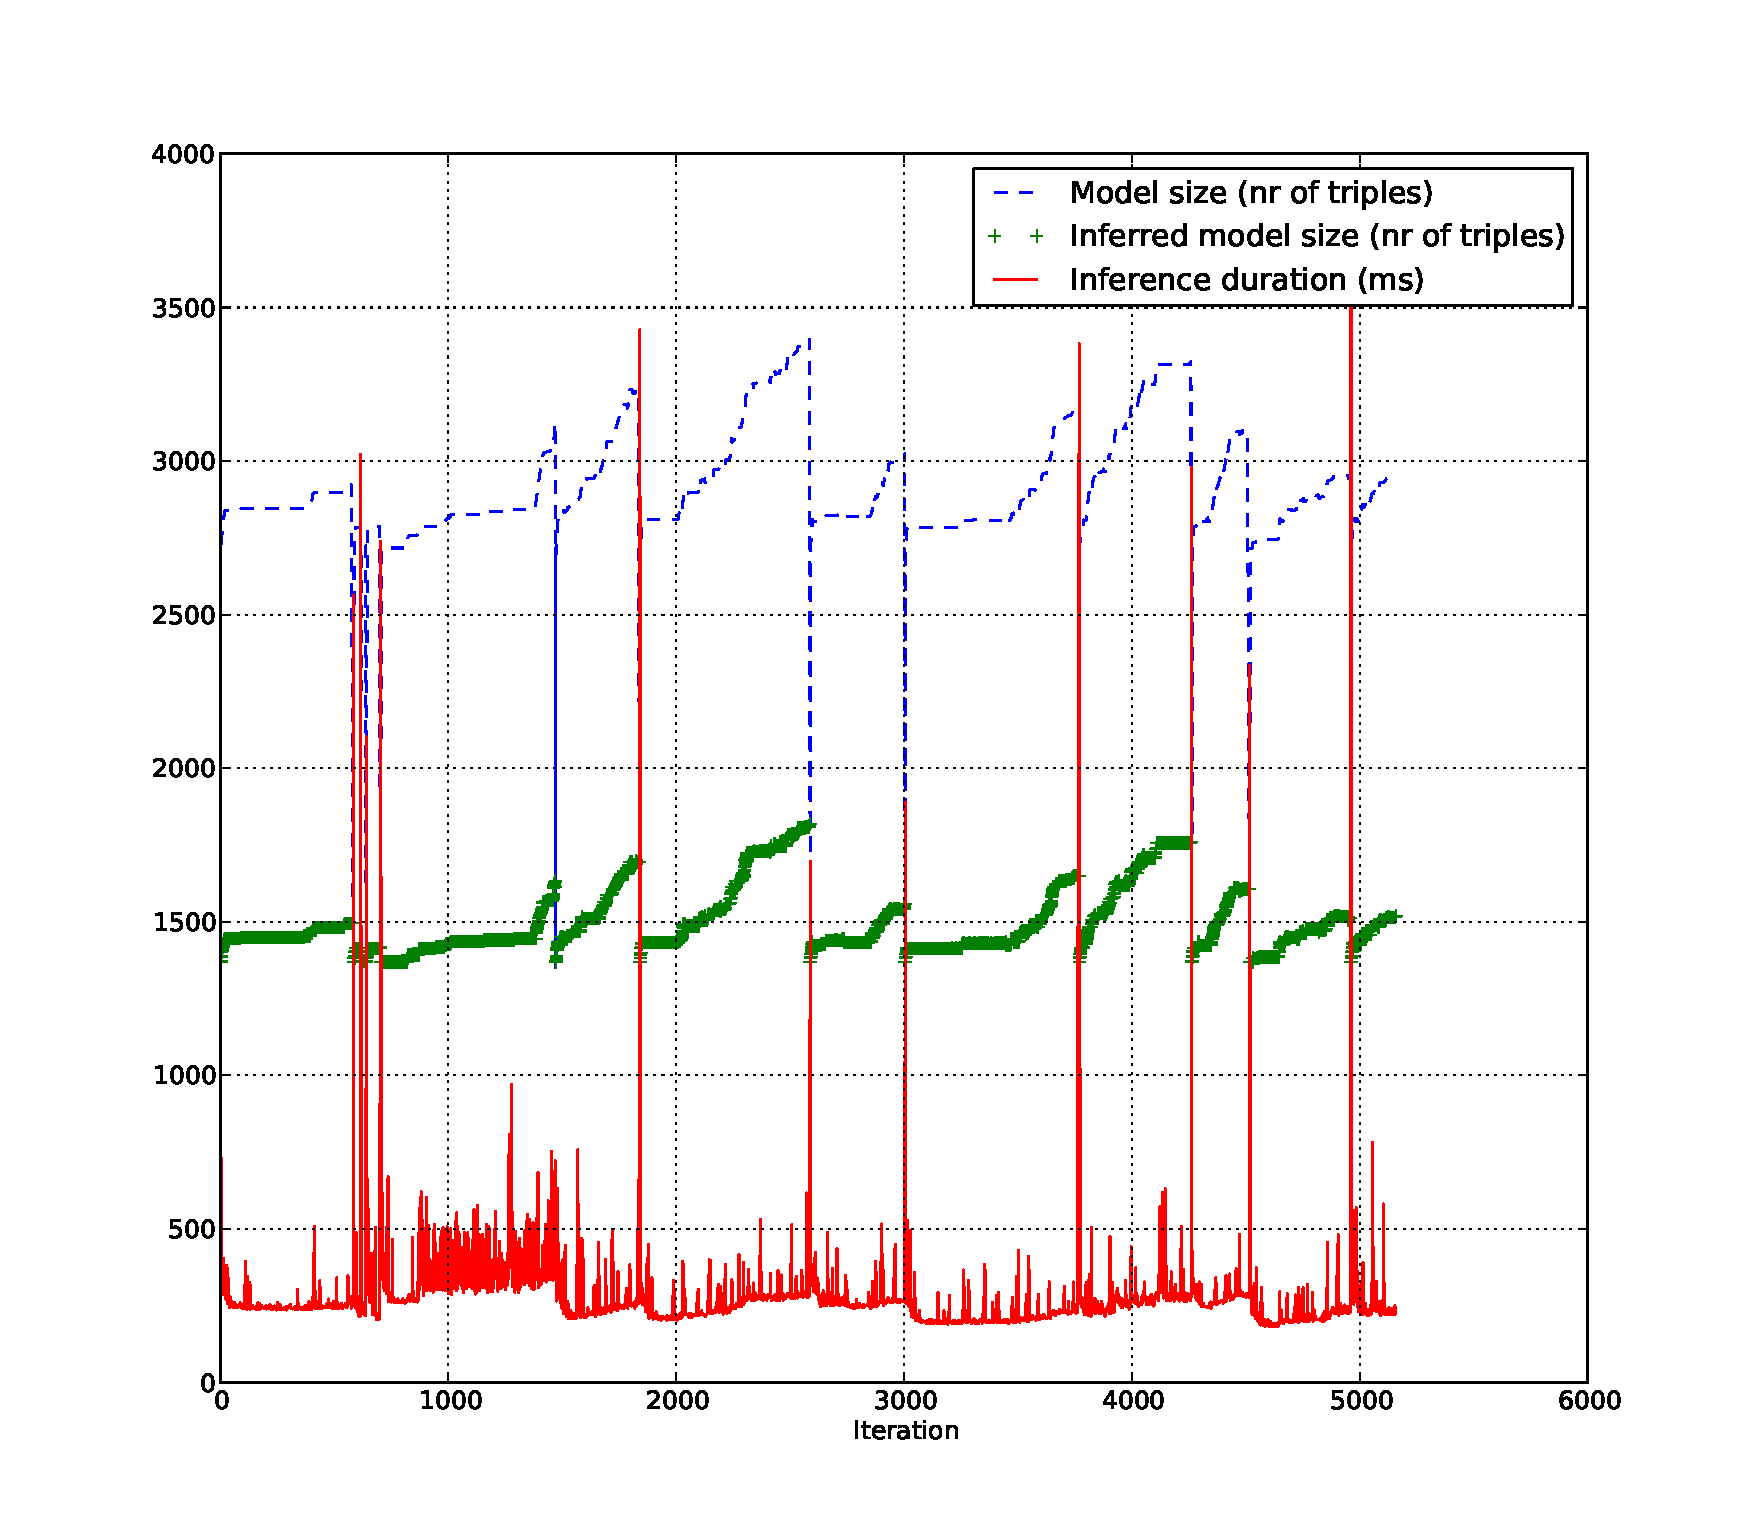
\includegraphics[width=450px]{stats}}
\caption{Size of asserted and inferred models for each iteration, including reasoning time}
\label{stats}
\end{figure}


\begin{table}
    \myfloatalign
  \begin{tabularx}{\textwidth}{lllllll} 
	\toprule
    \tableheadline{Component} & \tableheadline{Nr. of obs.} & \tableheadline{Min.} & \tableheadline{Max.} & \tableheadline{Mean} & \tableheadline{Std. dev.} \\ 
    \midrule

	Model size	& 5158 & 1346 &	3396 &	2916.7 & 201.07 \\
	Inferred model size &	5158 &	1369 &	1819 &	1501.8 & 107.6 \\
	Reasoning time & 5158 &	181 & 2912 & 274.99 & 152.96 \\
	
    \bottomrule
  \end{tabularx}
  \caption{Summary statistics for asserted and inferred model sizes and reasoning time}\label{summarySIB}
\end{table}


In Figure \ref{CPD}, the measurements show that the delay between the Presence-KP and the \ac{SIB} is rather large with a considerable variance. The communication from the Presence-KP to the \ac{SIB} consists of an update request and the related confirmation response. The average delay of 176.71 milliseconds is the largest component of the total end-to-end delay between the links. The communication from the \ac{SIB} to the Lamp-KP consists of an indication event from the \ac{SIB} due to a subscription and results in a query request from the Lamp-KP, terminated by a confirmation response by the \ac{SIB}. There is some variance in the communication delay and the average delay of 25.87 milliseconds might become problematic when the \ac{SIB} has to inform and handle multiple subscribers.

\begin{figure}
\centering
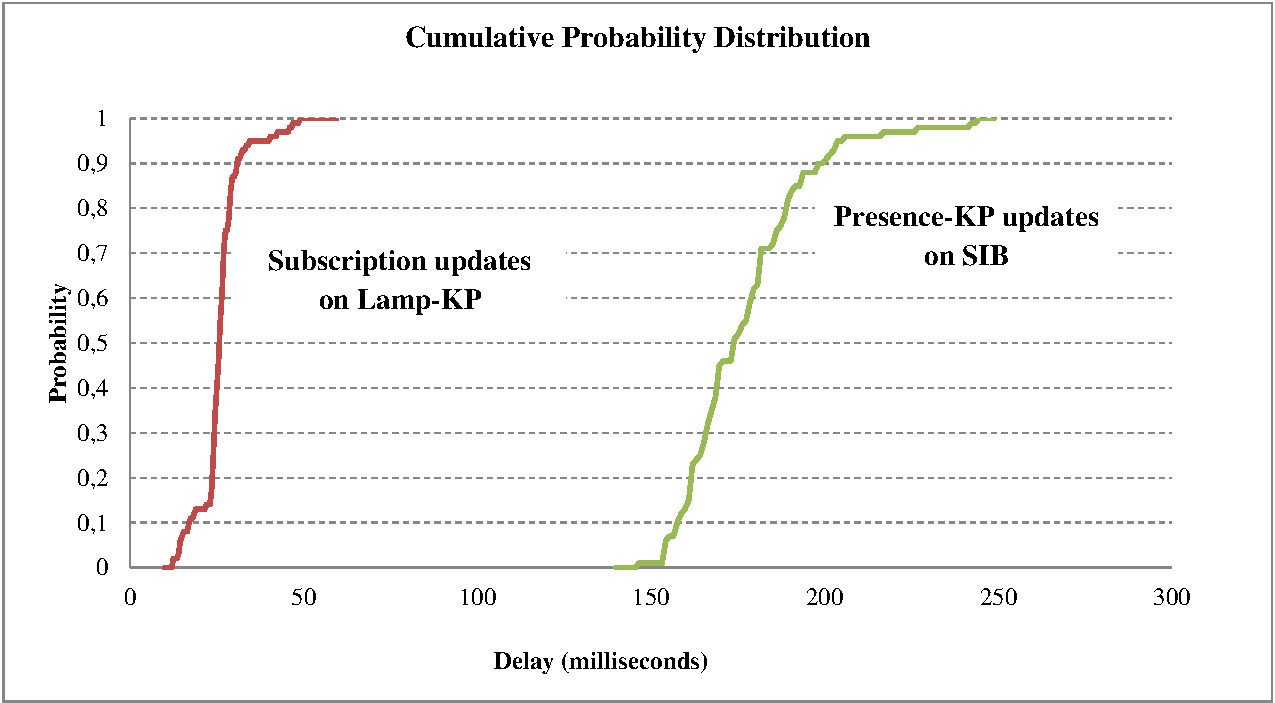
\includegraphics[width=\textwidth]{CPD}
\caption{Cumulative probability distribution of delays between Presence-KP and SIB, as well as SIB and Lamp-KP}
\label{CPD}
\end{figure}

\subsection{Discussion}

During the pilot, most problems could be attributed to problems with the wireless network. A number of devices from different manufacturers experienced intermittent problems while connected to the \ac{SIB}. For the purposes of the pilot, these devices were then connected to the \ac{SIB} via ethernet. This does, however, demonstrate some of the problems with existing wireless networking technologies. It cannot be expected that a device with a wireless connection will always stay connected to the smart space, even when it is within range of the wireless router.

%During one stakeholder visit, the comment was made that what we term semantic transformers, could also be termed transcoders, as they transcode data from one source type to another. With a large number of stakeholder visits the similarities of the SOFIA system to Universal Plug \& Play (UPnP) were discussed. It was pointed out that uPnP only covers one domain, and that it does not allow for the same type of device and capability descriptions on the semantic level.

If we compare our query time measurements to the ones performed on Smart-M3 (4.4ms) and \ac{RIBS} (0.65ms), we can see that the \acp{KP} were substantially slower: The Connector \ac{KP} at 44ms, the Music Player \ac{KP} at 74ms and the Sound/Light \ac{KP} at 60ms. This can be attributed to additional network latency in the field study that approximated a real-world environment. Query measurements that were performed on the ADK-SIB directly (0.445ms) shows that it performs even better than \ac{RIBS}, but this is not directly comparable as the measurements do not include network latency time. If network latency is taken into account, measured at 0.43ms per packet round-trip by \cite{Etelapera2011}, \ac{RIBS} is still faster.

The subscription indication measurements of our setup are also significantly slower. While the Smart-M3 measurement was only 140ms, the Music Player \ac{KP} measures around 860ms. This is mostly due to the additional time required for reasoning, which on average takes about 275ms. Reasoning improves the flexibility and capabilities of the \ac{SIB} to such an extent that it is worth the hit in performance. Other contributing factors include the number of devices used, the number of triples and the network environment. While the Smart-M3 and \ac{RIBS} measurements were made in a lab environment, our ADK-SIB measurements were made in conditions that approximate a real-world environment, including having a larger number devices active at the same time.

In the 1960s there already existed some controversy over the maximum allowable response times in human-computer interfaces \cite{Miller1968}. It was shown that different human actions will have different acceptable response times. While the delay between pressing a key and visual feedback should be no more than 0.1-0.3 seconds, the response to a inquiry request may take up to 2 seconds. The performance measurements are still well within this two-second limit, indicating that from a user's point of view, when performing routine tasks, the system is responsive enough. The user study and interviews performed during the pilot seem to confirm this, as no participant indicated any issues with regards to the responsiveness of the system.

The scalability of the system could still be evaluated with larger triple sizes, but we do not foresee any scalability issues, due to the platform and software architecture used. 

Not only the software architecture described in this thesis should be evaluated, but also the ontology that was developed during the three design iterations. This is the focus of the next section.

%When addressing another human being, we expect some communicative response between two and four seconds - any longer delay breaks the thread of communication and becomes embarrassing.


%SeNAmI end


\section{Evaluating the ontology}

\subsection{Introduction}

%Possobile TODO
% A variety of methods have been proposed \cite{DAquin2011} to evaluate ontology quality:
% 
% \begin{itemize}
% 	\item Testing and assessing the formal properties, e.g. using OntoClean \cite{Guarino2002}
% 	\item Using ontology design patterns (see Section \ref{DesignPatterns})
% 	\item Using unit tests as employed in software engineering
% 	\item Using opinions and rating using crowd-sourcing
% 	\item Using automatically generated metrics
% \end{itemize}

In the book Beautiful Data \cite{Segaran2009}, the notion of beauty is described as ``a simple and elegant solution to some kind of problem''. In a paper on the notion of beauty when building and and evaluating ontologies, D'Aquin and Gangemi \cite{DAquin2011} argue that the GoodRelations\footnote{http://www.heppnetz.de/projects/goodrelations/}\label{goodrelations} e-commerce ontology could be considered an example of a beautiful ontology. GoodRelations is an \ac{OWL} 1 DL ontology that is used by stores to describe products and their prices and features. Companies using the ontology include, Google, BestBuy, Sears, K-Mart and Yahoo. It addresses a complex domain and covers many of the complex situations that can occur in the domain. It is well designed, ontologically consistent, lightweight and used extensively by practitioners in the domain. 

Hepp \cite{Hepp2007}, creator of the GoodRelations ontology, describes a number of characteristics that can be used to evaluate an ontology:

\begin{itemize}
	\item High expressiveness: An ontology of higher expressiveness would be richly axiomatised in higher order logic, while a simple vocabulary would be of low expressiveness.
	\item Large size of community: As ontologies are considered community contracts, \marginpar{For more on community contracts, see Section \ref{CommunityContract}.} an ontology targeted towards a large community should be easy to understand, well doc\-u\-ment\-ed and of a reasonable size.
	\item Small number of conceptual elements: A larger ontology is more difficult to visualise and review. A reasoner could also take a long time to converge when the ontology is very large.
	\item Low degree of subjectivity: This is very much related to the domain of the ontology, where something like religion would be more subjectively judged than engineering.
	\item Average size of specification per element: The number of axioms or attributes used to describe each concept influences the ontological commitment\label{OntologicalCommitment} that must be made before adopting the ontology. %\marginpar{Ontological commitment relates to \emph{premature commitment}, which is described in more detail in Section TODO on the Cognitive Dimensions framework.}
\end{itemize}

We consider our ontology to be of higher expressiveness compared to other ubiquitous computing ontologies. Most of the existing technologies try to describe a large number of concepts, while the number of actual axioms used to describe these concepts are rather low. The size of the community is small at the moment, as only project partners in the \ac{SOFIA} project and students have been using the ontology up to now. Although the final version of our ontology contains 1192 asserted triples, the number of conceptual elements are low. There are only 34 \ac{OWL} classes, 29 object properties, 7 datatype properties and one magic property, making the ontology easy to visualise and review. Based on our experiments as described in the previous, the ontology also converges in a reasonable amount of time.

We now look at a method we developed to evaluate ontologies using the \ac{CD} framework, a framework that has been used to evaluate notational systems and programming environments \cite{Green1996}, and has also been used to evaluate two of the related projects described in Section \ref{RelatedProjects}: AutoHAN \cite{Blackwell2001} and e-Gadgets \cite{Mavrommati2004}.

\subsection{Validating the work using Cognitive Dimensions}
\label{CognitiveDimensions}

The \ac{CD} framework is a broad-brush approach to evaluating the usability of interactive devices and non-interactive notations, e.g. programming languages and \acp{API}. It establishes a vocabulary of terms to describe the structure of an artefact and shows how these terms can be traded off against each other. These terms are, at least in principle, mutually orthogonal.

Traditional HCI evaluation techniques focus on 'simple tasks' like deleting a word in a text editor, or trying to determine the time required to perform a certain task. They are not well suited to evaluating programming environments or notational issues. The \ac{CD} framework has been used to perform usability analyses of visual programming environments \cite{Green1996} as well as \acp{API} \cite{Clarke2004}. Mavrommati et al. \cite{Mavrommati2004} used the framework to evaluate the usability of an editing tool that is used to manage device associations in a home environment.

Microsoft \cite{Clarke2004} used the \ac{CD} framework to evaluate \ac{API} usability, as part of a user-centred design approach to \ac{API} design. Every \ac{API} has a set of actions that it performs. However, developers browsing the \ac{API} might not comprehend all the possible actions that the \ac{API} offers. In a usability study they asked a group of developers to use an API to perform a set of tasks, and then asked a set of questions for each dimension. For example, for role expressiveness(see Section \ref{cdDef}), the question was posed that when reading code that uses the \ac{API}, if it was easy to tell what each section of the code does and why.

For our evaluation, we focused on a subset of cognitive dimensions that are related to ubiquitous computing ontologies and systems. What follows is a list of these dimensions, including a short description where necessary, as well as an example question.


\begin{description}
  \item[Levels of abstraction] 	\label{cdDef}
	An abstraction is a grouping of elements that is treated as one entity, either for convenience or to change the conceptual structure \cite{Green1996}. \emph{What are the minimum and maximum levels of abstractions?}
    \item[Closeness of mapping] \emph{How clearly did the available components map onto the problem domain?}
	\item[Consistency] \emph{When some part of the ontology has been learnt, how much of the rest can be inferred by the developer? Where there were concepts in the ontology that mean similar things, is the similarity clear from the way they appear?}
	\item[Viscosity] To solve problems of viscosity, usually more abstractions (see earlier definition) are introduced in order to handle a number of components as one group, for example in object-oriented programming \cite{Green1996}. An example of viscosity is where it is necessary to make a global change by hand because the environment used does not have a global update tool. \emph{How much effort was required to make a change to the environment?}
	\item[Role expressiveness]
		The dimension of role expressiveness is intended to describe how easy it is determine what a certain part is for. \emph{Are there parts of the ontology that are particularly difficult to interpret?}
	\item[Hard mental operations] \emph{Are there places where the developer needs to resort to fingers or pencilled annotation to keep track of what is happening? What kind of things required the most mental effort with this system and ontology?}
	\item[Error-proneness] \emph{Did some kinds of mistakes seem particularly common or easy to make?}
	\item[Hidden dependencies] \emph{If some parts were closely related to other parts, and changes to one may affect the other, are those dependencies visible? }
\end{description}


 
% \subsection{Progressive evaluation}
% \label{progressive}
% For novices, it should be easy to check a program fragment before adding to it \cite{Green1996}. A partially-complete program should have the ability to be executed to obtain feedback on whether the developer has implemented new functionality correctly.


\subsection{Method}

The original \ac{CD} questionnaire \cite{Blackwell2007} was adapted for use with ubiquitous computing ontologies. Non-relevant questions were eliminated and some wording and questions were adjusted to the subject matter, without changing the fundamental meaning of the questions themselves. 

\marginpar{As mentioned in Section \ref{InteractionPrimitives}, our academic partners in Bologna published a journal paper \cite{Bartolini2011} based on an independent implementation of our work.}
Developers of the \ac{SOFIA} smart home pilot completed the questionnaire, as well as students and developers affiliated to the University of Bologna, for a total of 17 correspondents. The \ac{SOFIA} developers used the ontology and software architecture for a couple of weeks in order to construct the smart home pilot. The students in Bologna took part in a course based on technology developed within the \ac{SOFIA} project, where they also made use of the ontology and software architecture. 

Three additional questions not directly related to the cognitive dimensions, but meant to elicit more general responses about the usability of the ontologies and the system, were included in the questionnaire.

\begin{figure}[bth] 
        \subfloat[Background of correspondents]
        {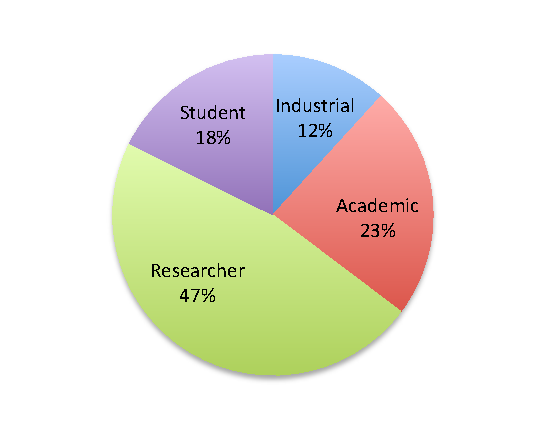
\includegraphics[width=.45\linewidth]{background}} \quad
        \subfloat[Correspondents' experience with software engineering and programming]
        {\label{experience}%
         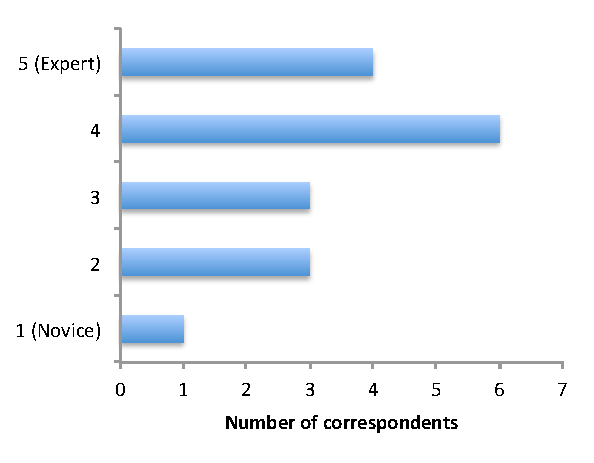
\includegraphics[width=.45\linewidth]{experience2}} \\
        \subfloat[Correspondents' experience with ontologies and semantic technologies]
        {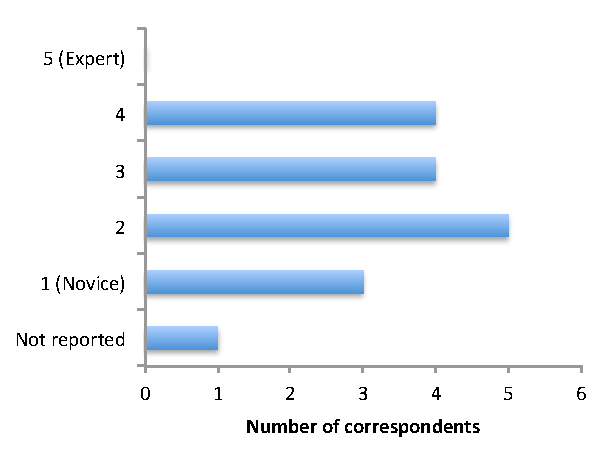
\includegraphics[width=.45\linewidth]{expOntologies2}} \quad
        
        \caption{Correspondent demographics}\label{demographics}
\end{figure}

% \begin{figure}
%         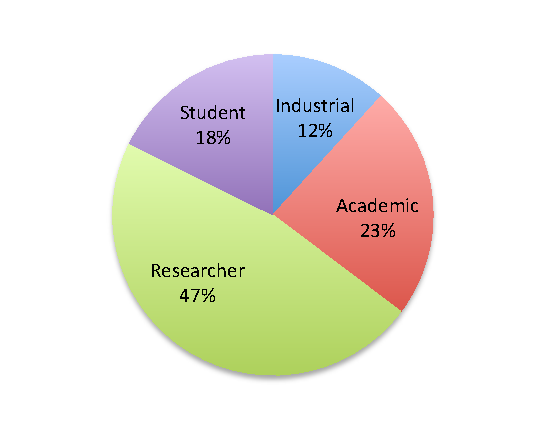
\includegraphics[width=250px]{background}
%         \caption{Background of correspondents}
% 		\label{background}
% \end{figure}
% 
% \begin{figure}[bth]
%         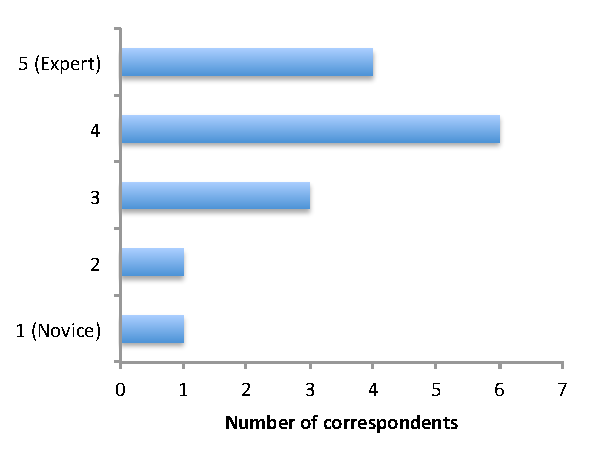
\includegraphics[width=.45\linewidth]{experience}
%         \caption{Correspondents' experience with software engineering and programming}
% 		\label{experience}
% \end{figure}
% 
% 
% \begin{figure}[bth]
%         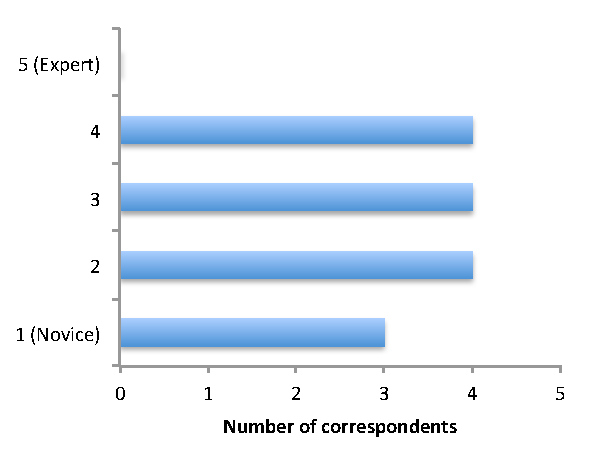
\includegraphics[width=.45\linewidth]{expOntologies}
%         \caption{Correspondents' experience with ontologies and semantic technologies}
% 		\label{expOntologies}
% \end{figure}

\subsection{Results}


\subsubsection{Levels of abstraction}
\label{LevelsOfAbstraction}
\begin{quote}
	\emph{Were you able to define your own concepts and terms using the system and ontology? Did you make use of different levels of abstraction?} An abstraction is a grouping of elements to be treated as one entity. In the ontology, these are defined as superclasses and subclasses, e.g. \texttt{PlayEvent} is a subclass of \texttt{MediaPlayerEvent}. Please indicate to what extent you made use of different levels of abstraction. If you did not use it, please indicate why.
\end{quote}

Most developers were able to make use of the existing concepts as defined, where the definition included different abstraction levels. Where necessary, developers were able to define their own concepts using different abstraction levels. Some of the developers used a simple ontology that did not require different levels of abstraction. As the level of knowledge about ontologies differed between different parties working on the same project, this necessitated the simplification of the ontology to a schema without semantics in some cases. Others avoided ontological reasoning altogether by embedding the logic in the \ac{KP} itself.


\subsubsection{Closeness of mapping}
\label{resultsCloseness}

\begin{quote}
	\emph{How clearly did the available components map to the problem domain?}
	Did you have to define any of your own components, or were any special tricks needed to accomplish specific functionality?
\end{quote}


Most of the developers experienced a clear, consistent mapping, with the domain mapped to already available components. In a few cases, developers developed their own components.

While it was easy to achieve the required functionality, it remains difficult to achieve component re-use. This becomes problematic for achieving emergent intelligent behaviour. 
It was also stated that more detailed descriptions of device capabilities, for example the coverage area of a presence sensor, are required.


\subsubsection{Consistency}

\begin{quote}
	\emph{Where there were concepts in the ontology that mean similar things, is the similarity clear from the way they appear?}
	Are there places where some things ought to be similar, but the ontology defines them differently? Please give examples.
\end{quote}

Most developers thought that similar entities in the ontology were subclassed correctly. It was indicated that \texttt{owl:sameAs} may be useful to indicate that different terms with the same meaning are in fact the same thing.

Afterwards we realised that developers not well acquainted with ontologies found it difficult to understand the difference between declaring entities using \texttt{rdfs:sub\-Class\-Of} and declaring them as individuals or instances, as well as how to model an entity that contains another entity.

Similar entities were not always instantiated in the same way, for example no state information was available for some smart objects.
Where multiple domain ontologies with similar concepts were used, these concepts were not aligned - most developers expected some upper (or core) ontology to align and unify main concepts.
Concepts need a clear textual description and usage examples to make them easier to understand.

\subsubsection{Viscosity}

\begin{quote}
	\emph{How much effort was required to make a change to the environment? Why?}
	How difficult is it to make changes to your program, the ontology or the system? For example, was it necessary to make a global change by hand because no global update tools were available?
\end{quote}

Although different domains used different terms to define ontological concepts, most developers found it quite easy to make changes for ontological agreement. However, changes to the ontology sometimes necessitated changes at code level. In most cases, it was easier to adapt to changes on a semantic level, as the \ac{KP} domain boundaries were well defined.

Using ontologies made it easier to allow for definition changes at run-time. Depending on the inferencing method used, changes to the ontology could require some existing inferences to be removed. 

One developer working with an embedded system found changes to be more difficult to implement, as it still required rebuilding images and downloading them to embedded boards for each modification. Some found it difficult to view changes made to the environment, due to a lack of tools to explore the contents of the \ac{SIB}.


\subsubsection{Role expressiveness}

\begin{quote}
	\emph{Are there parts of the ontology that are particularly difficult to interpret?}
	How easy is it to answer the question: 'What is this bit for?' Which parts are difficult to interpret?
\end{quote}

Most responses indicated that the ontology was easy to understand. More clarifying comments inside the ontology could be useful - this can be implemented using the \texttt{rdfs:comment} field. Some developers indicated that application ontologies (ontologies that are device-specific) were still hard to interpret. 

Some concepts might be instinctively interpreted differently, but the defined meaning became clear when viewed in context with the rest of the ontology. The ontology provides the structure that is necessary to make sense of the concepts.


\subsubsection{Hard mental operations}

\begin{quote}
	\emph{What kind of things required the most mental effort with this system and ontology?}
	Did some things seem especially complex or difficult to work out in your head (e.g. when combining several things)? What are they?
\end{quote}

Multiple developers indicated that ontologies are not an easy concept to grasp and that common practice is not always clear. Once familiar with ontologies, and understanding the specific ontologies involved, developers thought they were easy to use.  

There is still effort required to make the system adaptive. This issue is also mentioned in Section \ref{resultsCloseness}.


\subsubsection{Error-proneness}

\begin{quote}
	\emph{Did some kinds of mistakes seem particularly common or easy to make? Which ones?}
	Did you often find yourself making small slips that irritate you or make you feel stupid? What are some examples?
\end{quote}

Some developers found it quite easy to mistype string literals, indicating that it would be better to define entities to represent strings that occur more than once. Mistyping URIs was another common error, as well as mixing up namespaces. Developers not familiar with ontologies also mixed up or misunderstood the differences between URIs and literals.

\subsubsection{Hidden dependencies}

\begin{quote}
	\emph{If some parts were closely related to other parts, and changes to one may affect the other, are those dependencies visible?}
	What kinds of dependencies were hidden? How difficult was it to test the implemented system? Were there hidden faults that were difficult to find?
\end{quote}

Multiple developers noted that using ontologies made the relationships among entities/parts more visible. 

Changes to the ontology may affect others, therefore versioning and update notification are important. In the system used no errors were raised when components adhered to different versions of the ontology. Broken dependencies were only visible when the overall system failed.

One developer indicated that the publish/subscribe approach followed by the system architecture allowed for minimal dependencies due to loose coupling.

Some developers noted that it was difficult to determine when something did not work. This was especially noticeable in the case of subscriptions, were it becomes really difficult to understand why a certain subscription-based notification was not received.

One developer suggested that an ontology viewer could be used to make dependencies more visible, and that the Prot\'eg\'e ontology editor is too complex for most users.\marginpar{The Prot\'eg\'e ontology editor was first mentioned in Section \ref{D2Discussion}.}


\subsection{Non-CD related questions}

Some questions in the questionnaire were not directly related to the cognitive dimensions, but were meant to elicit more general responses to the usability of the ontologies and system.\\

\begin{cdquestion}
	What obstacles made it difficult to use the system?
\end{cdquestion}

This question was based on a survey done by \cite{Robillard2009} to determine aspects that make \acp{API} hard to learn. The question was phrased as follows:

\begin{quote}
\emph{What obstacles made it difficult for you to use the system?} Obstacles can have to do with the system itself, with your background, with learning resources etc. List the three most important obstacles, in order of importance (1 being the biggest obstacle). Please be more specific than the general categories mentioned here.
\end{quote}

Responses included:

\begin{itemize}
	\item Lack of background in ontologies
	\item Poor documentation
	\item Insufficient code examples
	\item \ac{SSAP} poorly documented\marginpar{\ac{SSAP} is described in more detail in Section \ref{ssap}.}
	\item Difficult setup and installation procedure
	\item Lack of proper tools for viewing and exploring contents of \ac{SIB}
	\item Reliability of subscription mechanism, especially on wireless networks
	\item QNames not supported on all platforms, requiring full \ac{URI} to be specified\marginpar{QNames enable full \acp{URI} to be substituted by short prefixes.}
	\item Ontology agreement
	\item Stability, performance, network issues
\end{itemize}
\vspace{0.5cm}


\begin{cdquestion}
	What did you appreciate most about the system and ontology?
\end{cdquestion}

Responses included:

\begin{itemize}
	\item Decoupling of interaction between components (i.e. all communication through broker, but could be single point of failure)
	\item Semantic interoperability between different devices, manufacturers and architectures
	\item Easy and quick to define new applications based on ontologies (after training)
	\item Using semantic connections to connect devices
	\item Ontology usable in different domains and more complex scenarios
	\item Ability to react to context changes through subscriptions
\end{itemize}


One respondent had the following insight: ``Once you have agreed on the ontologies and the KP's functionalities, you can focus on handling the various subscriptions and inserting the necessary triples. One does not have to focus on the communication protocols used or on the communication with the other components themselves.''\\


\begin{cdquestion}
	Can you think of ways the design of the system and ontology can be improved?
\end{cdquestion}

Responses included:

\begin{itemize}

	\item \ac{SIB} discovery
	\item Agreement on ontological concepts to be used by a technical group
	\item Tools for ontology design (currently external tools are required)
	\item Better documentation
	\item Self-description of UI concepts and component functionality 
	\item Hierarchic Smart Spaces
	\item Locality/routing/separation of message buses
	\item Authentication/security/locking
	\item Forcing a programming paradigm like \ac{OOP} influences semantic treatment
	\item How to handle faulty smart objects
\end{itemize}

\marginpar{These results were communicated by the author to the other project partners in the \ac{SOFIA} project at a review meeting.}

\subsection{Discussion}

% Every notation highlights some kinds of information at the expense of obscuring other kinds \cite{Green1996}. For example, rule-based languages highlight conditions under which certain actions are taken, while it hides the sequential ordering of these actions. There must also be a cognitive fit between the mental representation and external representation. For example, if your mental representation is in control flow form, a data flow language will be difficult to use. 

Ontologies allow developers to create additional levels of abstraction when the existing abstractions are not sufficient. The bigger issue seems to be unfamiliarity with ontologies, with some developers going so far as to embed all logic in the code itself in order to avoid using ontologies, as mentioned in Section \ref{LevelsOfAbstraction}.

For the ontologies we defined, there seems to be clear mapping between objects in the domain and the ontological entities that they are mapped to. Adding additional components where necessary did not present any problems. One area that needs more attention is the extending the level of detail for device capability descriptions. Keep in mind, however, that too many low-level primitives create a cognitive barrier to programming \cite{Green1996}. It is not easy to deal with entities in the program domain that do not have corresponding entities in the problem domain. For example, having many ways to describe a presence sensor, when only one or two of these are relevant to the problem domain, makes it more difficult for the developer to comprehend.

When creating an ontology, it is important to provide clear textual descriptions, clarifying comments and usage examples for concepts to make them easier to understand. The GoodRelations e-commerce ontology is a good example of how this can be achieved.\marginpar{GoodRelations was first discussed in Section \ref{goodrelations}.}

Tools to explore the contents of the triple store more efficiently could decrease viscosity, as it would simplify viewing changes made to the environment and make dependencies more visible. Existing ontology viewers are still considered complex to use, usually only by ontology experts. Tools to automatically detect namespaces and prevent mistyping of \acp{URI} and strings used in the ontology would also be very useful.

%There is still effort required to make the system adaptive in order to achieve emerging behaviour. There is not enough component re-use, which may be due to lack of knowledge of existing components and their behaviour. Existing components should be easy to repurpose and shared behaviour must be properly documented. 

In addition to the strengths and limitations of the software architecture and the ontology described in this chapter, we discuss more general conclusions and achievements in the next chapter.



% TODO
% - OntoClean
% - Aligning to DOLCE (DUL)
% 
% 
% TODO Compare with DLNA/UPnP as a case study
% 
% Possible TODO
% Compare to Logitech Harmony One Universal Remote Control (See Evernote)
% - Compare ontological approach to APIs http://itu.dk/stud/speciale/gamelib/APIUsability.pdf
% - Validate generalization of ontology (compared to existing ones)